% !TEX TS-program = latex  
\documentclass[english,dvipsnames]{beamer}     %  ,handout
\usepackage{babel}
\usepackage[utf8]{inputenc}
\usepackage{pgffor} 
\usepackage{listings}
\usepackage{graphicx}
\usepackage{algorithm}
\usepackage{algorithmic}
\usepackage{color, colortbl}
\usepackage[absolute,overlay]{textpos}
\usepackage{ bbold }
\usepackage[
  style=numeric,
  %autocite=footnote,
  maxnames=10,
  babel=hyphen,
  hyperref=true,
  abbreviate=false,
  backend=biber,
  doi=false,
  url=false,
  giveninits=true,
  isbn=false,
  indexing=true
  ]{biblatex}   

  \renewcommand{\algorithmicrequire}{\textbf{Input:}}
  \renewcommand{\algorithmicensure}{\textbf{Output:}} 
  \resetcounteronoverlays{algorithm}

\usepackage{standalone}
  \standaloneconfig{mode=image} % mode=buildnew OR mode=image %%%%%

\usepackage[T1]{fontenc}
\usepackage{multicol}
\usepackage{textcomp} % to get the right copyright, etc.
\usepackage{amsmath} % before lucidabr
\usepackage{tikz} 
  \usetikzlibrary{patterns}
  \usetikzlibrary{snakes}
\usetikzlibrary{arrows,decorations.markings}
\usetikzlibrary{positioning}
\usetikzlibrary{calc}


\setlength{\parskip}{0pt}%
\usepackage{soul}




% use Lucida fonts for both text and math.
% \usepackage[T1,altbullet,expert,nofontinfo,lucidascale]{lucidabr}     % get larger bullet
\DeclareEncodingSubset{TS1}{hlh}{1}  % including \oldstylenums
%%%%%
\addtobeamertemplate{footnote}{\vspace{-6pt}\advance\hsize-0.5cm}{\vspace{6pt}}
\makeatletter
\renewcommand*{\footnoterule}{\kern -3pt \hrule \@width 2in \kern 8.6pt}

\usetheme{Madrid}  % default minimalista

\usecolortheme{rose}

\newenvironment<>{problock}[1]{%
  \begin{actionenv}#2%
      \def\insertblocktitle{#1}%
      \par%
      \mode<presentation>{%
        \setbeamercolor{block title}{fg=white,bg=orange!20!black}
       \setbeamercolor{block body}{fg=black,bg=olive!50}
       \setbeamercolor{itemize item}{fg=orange!20!black}
       \setbeamertemplate{itemize item}[triangle]
     }%
      \usebeamertemplate{block begin}}
    {\par\usebeamertemplate{block end}\end{actionenv}}






\DefineBibliographyStrings{english}{%
  bibliography = {References},
}
\addbibresource{biblio.bib}
\renewcommand{\footnotesize}{\scriptsize}
%----------------------------------------------------------------------------%
\title[Universality and complexity of FCA] % (optional, only for long titles)
{Universalité et complexité \\ des automates cellulaires coagulants}

\subtitle{ \small Universality and complexity of freezing cellular automata}

\author[Diego Maldonado] % (optional, for multiple authors)
{Diego Maldonado}
 
\date{26 novembre 2018}
    
  

\subject{Computer Science}
\AtEveryCitekey{\iffootnote{\color{red}\scriptsize}{\color{blue}}}


\begin{document}
%-----------------------------------------------------------------------------------------------------------------------------------------%
\begin{frame}
  \begin{center}
 
\includegraphics[height=1.25cm]{./img/univ.png}\hfill 
\includegraphics[height=1.25cm]{./img/lifo.pdf}
  \end{center}
  \titlepage
\end{frame}
%-----------------------------------------------------------------------------------------------------------------------------------------%
%-----------------------------------------------------------------------------------------------------------------------------------------%
\begin{frame}
\frametitle{Intuition and Examples}

\begin{block}{}
  A behavior is ``Freezing'' if its state only ``decreases'' or ``follows one direction''.
\end{block}
\medskip
\centering
\pause
  \begin{minipage}[b]{0.4\textwidth}
    \centering
              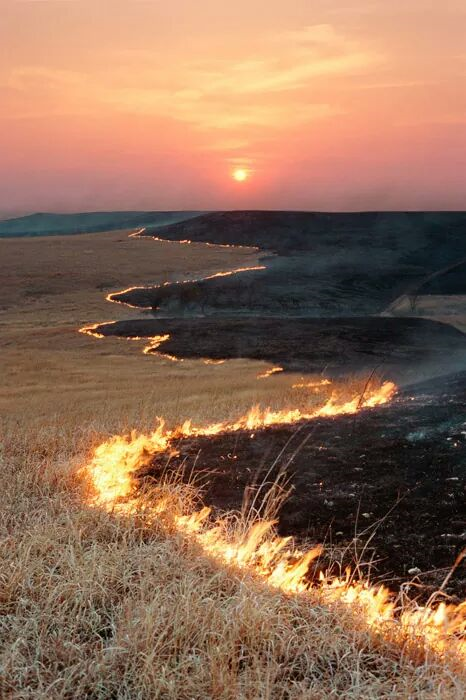
\includegraphics[height=3.5cm]{./img/FB.png} 
            \\ Forest Fire \pause
            \\ tree $\to$  fire $\to$ ash
  \end{minipage}\qquad\qquad\pause
    \begin{minipage}[b]{0.45\textwidth}
    \centering
    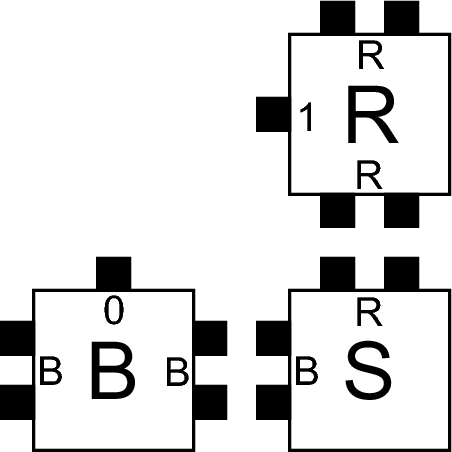
\includegraphics[height=2.5cm]{./img/seft.png}
    \\ Self-assembly tilings.  \pause   
    \\  empty  $\to$ tile 1, tile 2, ..., tile n
  \end{minipage}\pause

\end{frame}

%---------------------------------------------------------------------------------------------%
%-----------------------------------------------------------------------------------------------------------------------------------------%
\begin{frame}
\frametitle{Blocks}

\begin{block}{Block 0}
  Block
\end{block}
\medskip
\centering
\pause
\begin{minipage}[b]{0.4\textwidth}
  \begin{block}{Block 1}
    block
  \end{block}
\end{minipage}\pause\hfil
\begin{minipage}[b]{0.4\textwidth}
  \begin{block}{Block 2}
    block
  \end{block}
\end{minipage}

\end{frame}
%-----------------------------------------------------------------------------------------------------------------------------------------%
\begin{frame}
\frametitle{Remplazando blocks}

\alt<1-2>{
  \begin{block}{Block 0}
    Block
  \end{block}
}{
  \begin{alertblock}{Block 3}
    Block nuevo
  \end{alertblock}
}

\medskip
\centering
\uncover<2->{
\begin{minipage}[b]{0.4\textwidth}
  \begin{block}{Block 1}
    block
  \end{block}
\end{minipage}
}
\hfil
\uncover<3->{
\begin{minipage}[b]{0.4\textwidth}
  \begin{block}{Block 2}
    block
  \end{block}
\end{minipage}
}
\end{frame}
%---------------------------------------------------------------------------------------------------------------------------------------%
\begin{frame}
\frametitle{Cite}


  \begin{block}{Block 0}
    Block \footfullcite{FUCA18}
  \end{block}

\end{frame}

%---------------------------------------------------------------------------------------------%



\begin{frame}
\begin{center}
\alt<1>{
\includestandalone[height=.2\textheight]{./img/cuadrado}}
{\includestandalone[height=.2\textheight]{./img/cuadrado1}}
\uncover<3->{
\includestandalone[height=.2\textheight]{./img/flecha}
\includestandalone[height=.2\textheight]{./img/cuadrado2}
}
\uncover<4->{
\includestandalone[height=.2\textheight]{./img/flecha}
\includestandalone[height=.2\textheight]{./img/puntos}
\includestandalone[height=.2\textheight]{./img/flecha}
\includestandalone[height=.2\textheight]{./img/cuadrado3}
}

\begin{minipage}[b]{0.4\textwidth}
  \begin{alertblock}{}
    block \alert{algo importante}
  \end{alertblock}
\end{minipage}
\end{center}


\end{frame}

%---------------------------------------------------------------------------------------------%
  
\begin{frame}[t,allowframebreaks]
  \frametitle{References}
  \printbibliography[heading=subbibliography  ,title={References}]
  \vspace{25pt}

 \end{frame}
%---------------------------------------------------------------------------------------------%
\begin{frame}

\vfil
  
  \begin{center}
  \Huge \bf ¡Muchas Gracias!
  \end{center}
\end{frame}
\end{document}
